\documentclass[a4paper,12pt]{article}
\usepackage [utf8]{inputenc}
\usepackage [italian]{babel}
\usepackage{graphicx}
%\usepackage{grffile}
\usepackage{listings}
\usepackage{color}
\usepackage[hidelinks]{hyperref}
\usepackage{calc}

\addtolength{\oddsidemargin}{-30pt}
\addtolength{\textwidth}{60pt}
\addtolength{\voffset}{-60pt}
\addtolength{\textheight}{100pt}


\graphicspath{ {../Schema concettuale} {../Schema logico relazionale} {../Piani di accesso} }
\lstset{inputpath=../Sorgenti SQL/}

\definecolor{codegreen}{rgb}{0,0.6,0}
\definecolor{codegray}{rgb}{0.5,0.5,0.5}
\definecolor{codepurple}{rgb}{0.58,0,0.82}
\definecolor{backcolour}{rgb}{0.95,0.95,0.92}

\lstdefinestyle{mystyle}{
    language=SQL,
    backgroundcolor=\color{backcolour},   
    commentstyle=\color{codegreen},
    keywordstyle=\color{magenta},
    numberstyle=\small\color{codegray},
%    xleftmargin=-10px,
    stringstyle=\color{codepurple},
    basicstyle=\ttfamily,
    breakatwhitespace=false,         
    breaklines=true,                 
%    captionpos=b,                    
    keepspaces=true,                 
    numbers=left,                    
    numbersep=10pt,                  
    showspaces=false,
    showstringspaces=false,
    showtabs=true,
    tabsize=4
}
\lstset{style=mystyle}

\addto\captionsitalian{%
\renewcommand{\lstlistingname}{Codice}}
\addto\captionsitalian{%
\renewcommand{\lstlistlistingname}{Elenco dei listati di codice}}


%%%%%%%%%%%%%%%%%%%%%%%  FRONTESPIZIO %%%%%%%%%%%%%%%%%%%%%%%

\title { \vspace{-1.0cm}{\small Università di Pisa\\Dipartimento di Informatica\\Corso di Laurea in Informatica\\[0.5cm]Corso di Basi di Dati (244AA), prof. Giorgio Ghelli\\[0.7cm]}Progetto ``Studio professionale fatture"\\Relazione finale }
\author { Candidato:\\Alessandro Antonelli\\(matricola 507264, corso A) }
\date { Consegna: 24 marzo 2021\\Appello straordinario marzo 2021\\A.A. 2019/2020 }

\begin {document}
 \maketitle
 
 \tableofcontents

\listoffigures

\lstlistoflistings

 \clearpage
 
%%%%%%%%%%%%%%%%%%%%%%%  CONTENUTO %%%%%%%%%%%%%%%%%%%%%%%

 \section{ Descrizione del dominio }

Bla bla bla

 \section{ Schema concettuale }

\begin{figure}[h]
    \centering
    \caption{Schema concettuale a oggetti}
    \centerline{
	 \frame{
      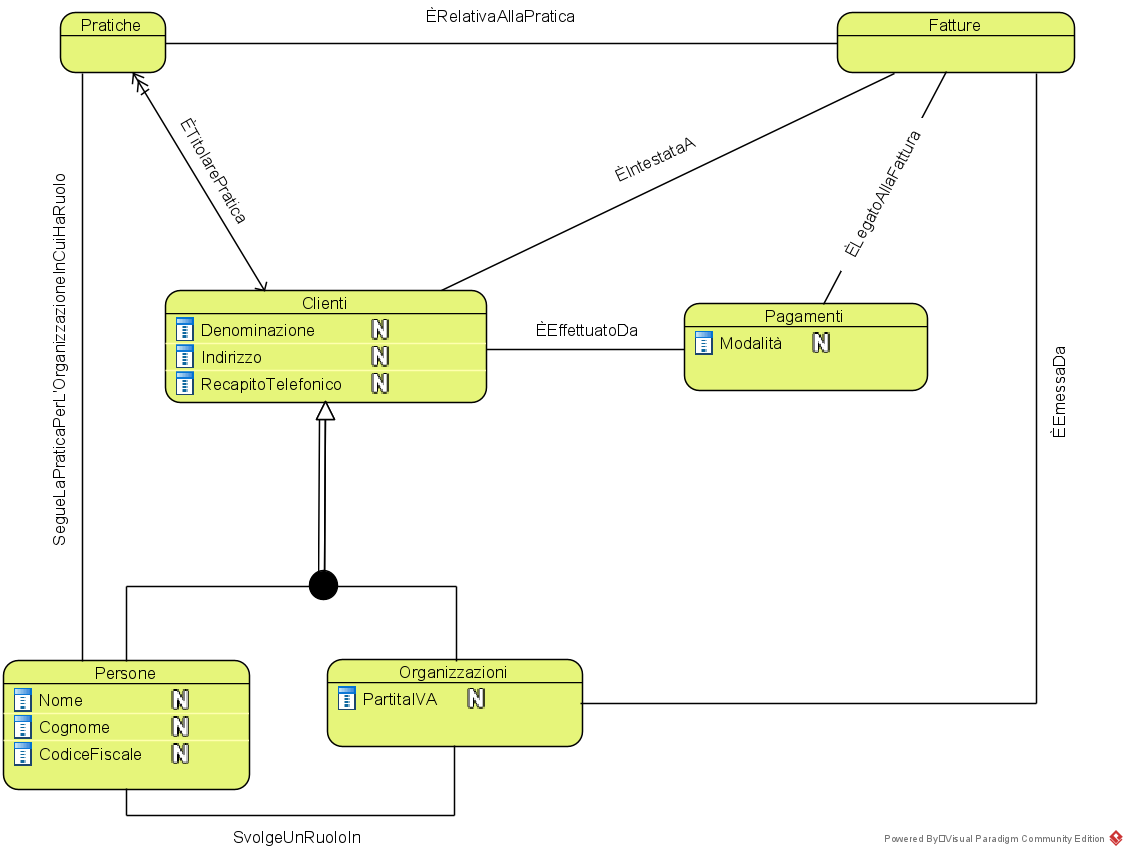
\includegraphics[width=\paperwidth-1cm]{ Schema concettuale a oggetti.png }
    } }
    \label{GraficoConcettuale}
\end{figure}

%nel testo, per indicare il numero di figura, si può usare \ref{} scrivendo tra le graffe il contenuto di "label"

 \subsection{ Vincoli }

 \subsection{ Vincoli intrarelazionali }

 \subsection{ Vincoli interrelazionali }

 \section{ Schema logico relazionale }

 \subsection{ Formato grafico }

 \subsection{ Formato testuale }

 \subsection{ Dipendenze funzionali }

 \subsubsection{ Relazioni A, B, C }

 \subsubsection{ Relazioni C, D, E }

 \subsubsection{ Relazioni X }

 \section{ Interrogazioni }

 \subsection{ Uso di proiezione, join e restrizione }
 \subsection{ Uso di group by con having, where e sort }
 \subsection{ Uso di join, group by con having e where }
 \subsection{ Uso di select annidata con quantificazione esistenziale }
 \subsection{ Uso di select annidata con quantificazione universale }
 \subsection{ Uso di subquery di confronto quantificato usando una subquery }

\lstinputlisting[caption=esempio]{esempio.sql}

 \section{ Piani di accesso }

 \subsection{ Piani di accesso logico }

 \subsubsection{ Query 1) }

 \subsubsection{ Query 2) }

 \subsubsection{ Query 3) }

 \subsection{ Piani di accesso fisico senza uso di indici }

 \subsubsection{ Query 1) }

 \subsubsection{ Query 2) }

 \subsubsection{ Query 3) }

 \subsection{ Piani di accesso fisico con uso di indici }

 \subsubsection{ Query 1) }

 \subsubsection{ Query 2) }

 \subsubsection{ Query 3) }

\end{document}